Pour cette gamme de simulation, nous avons choisi de revenir sur un jeu de conditions proche de notre première idée. Nous allons plonger une sphère de Hénon dans un bain homogène remplissant une boîte.
La première chose à faire est de stabiliser le cube. Mais présentons d'abord le système d'unité utilisé ici.

\subsection{Système d'unité}
	Nous nous plaçons dans le système décrit dans \cite{fuji1983}. C'est à dire:
	\begin{itemize}
		\item $\tilde{M_h} = 1$
		\item $\tilde{R_0} = 2$
		\item $\tilde{G} = 1$
	\end{itemize}

	Le changement de variable a effectué pour passer des unités physiques à celle de l'article est le suivant:
	\begin{align}
		\begin{cases}
			\tilde{m} = \frac{m}{M_t} \\
			\\
			\tilde{r} = \frac{r}{R_0} \\
			\\
			\tilde{v} = \frac{v}{\sqrt{\frac{GM_t}{R_0}}}
		\end{cases}
	\end{align}
	Point intéressant, le temps dynamique devient:
	\begin{align}
		T_d = \pi \sqrt{\frac{R_0^3}{2GM}} = 2\pi
	\end{align}

\subsection{Stabilité du cube}
	\begin{wrapfigure}{l}{0.20\textwidth}
		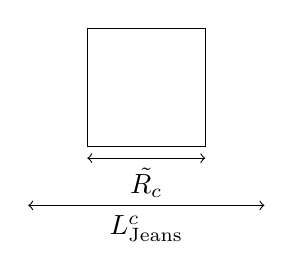
\begin{tikzpicture}[scale=1.5]
			\draw (0, 0) -- (1, 0) -- (1, 1) -- (0, 1) -- (0, 0);
			\draw[<->] (0, -0.1) -- (1, -0.1);
			\draw (0.5, -0.1) node[below] {$\tilde{R_c}$};
			\draw[<->] (-0.5, -0.5) -- (1.5, -0.5);
			\draw (0.5, -0.5) node[below] {$L_\mathrm{Jeans}^c$};
		\end{tikzpicture}
	\end{wrapfigure}
	Vouloir faire une simulation avec un cube interagissant, c'est bien beau, mais un tel objet risque de s'effondrer plutôt vite. Il va nous falloir une condition pour pouvoir le stabiliser.
	Une sphère homogène est stable si sa taille est inférieur à sa longueur de Jeans. Notre critère est donc le suivant:
	\begin{align}
		\tilde{R_c} &< L_\mathrm{Jeans}^c = \frac{\sigma_c}{\sqrt{GM_c}} \notag \\
		\tilde{R_c}^2 &< \frac{\sigma_c^2}{GM_c} \notag \\
		GM_c\tilde{R_c}^2 &< \sigma_c^2
	\end{align}
	Nous imposons aux particules du cube d'avoir la même masse que celle du Hénon, soit:
	\begin{align*}
		m_c = m_h = \dfrac{M_h}{N_h}
	\end{align*}
	où $N_h$ est le nombre de particules du Hénon. Soit $N_c$ le nombre de particules du cube,
	notre critère devient:
	\begin{align}
		GM_h\dfrac{N_c}{N_h}\tilde{R_c}^2 &< \sigma_c^2 \notag \\
		\dfrac{N_c}{N_h}\tilde{R_c}^2 &< \sigma_c^2 \\
		\dfrac{N_c}{N_h} &< \dfrac{\sigma_c^2}{\tilde{R_c}^2}
	\end{align}
	en oubliant pas que: $G=1$ et $M_h=1$.

\subsection{Conditions de la simulation}
	Comme nous cherchons à vérifier notre modèle, nous devons placer le bain à une température
	inférieur à celle que la sphère de Hénon atteint une fois à l'équilibre. Soit $\sigma_h^f$ la
	dispersion de vitesse de la sphère après effondrement, on doit avoir:
	\begin{align}
		\sigma_c &< \sigma_h^f \notag
	\end{align}

